\documentclass[a4paper,10pt]{article}

\usepackage{natbib}
\usepackage{amsthm}
\usepackage{amsfonts}
\usepackage{amssymb}
\usepackage{amsmath}
\usepackage{latexsym}
\usepackage{graphicx}
\usepackage{blindtext}
\usepackage{float}

\usepackage{doc}

\renewcommand{\figurename}{Obr.}

\setcitestyle{square}

\newtheorem*{theorem}{Theorem}
\theoremstyle{definition}
\newtheorem*{definition}{Definition}

\hoffset -1in \topmargin 0mm \voffset 0mm \headheight 0mm
\headsep0mm
\oddsidemargin  20mm     %   Left margin on odd-numbered pages.
\evensidemargin 20mm     %   Left margin on even-numbered pages.
\textwidth   170mm       %   Width of text line.
\textheight  252mm

\makeatletter
\renewcommand\@openbib@code{%
     \advance\leftmargin  \z@ %\bibindent
      \itemindent \z@
     % Move bibitems close together
     \parsep -0.8ex
     }
\makeatother

\makeatletter
\renewcommand\section{\@startsection {section}{1}{\z@}%
                                   {-3.5ex \@plus -1ex \@minus -.2ex}%
                                   {1.5ex \@plus.2ex}%
                                   {\large\bfseries}}
\makeatother

\makeatletter
\renewcommand\subsection{\@startsection {subsection}{1}{\z@}%
                                   {-3.5ex \@plus -1ex \@minus -.2ex}%
                                   {1.5ex \@plus.2ex}%
                                   {\normalsize\bfseries}}
\makeatother

\makeatletter
	\setlength{\abovecaptionskip}{3pt}   % 0.25cm 
	\setlength{\belowcaptionskip}{3pt}   % 0.25cm 
\makeatother

\begin{document}
\pagestyle{plain}

\begin{center}
{\bf \Large ROBOTIZACE A AUTOMATIZACE VE ZPRACOVÁNÍ ODPADU}
\end{center}

\smallskip
\begin{center}
{\large Autor: Lukáš Jiroušek}
\end{center}

\smallskip
\begin{center}
Fakulta strojního inženýrství, Vysoké učení technické v Brně\\
Ústav automatizace a informatiky\\
Technicka 2896/2, Brno 616 69, Česká republika\\
208696@vutbr.cz\\
\end{center}

\bigskip
\noindent Abstrakt: \textit{Tato práce se zabývá robotizací a automatizací průmyslu pro zpracování odpadu. To od jeho sběru až po metody třídění. Tradičně se tomuto věnovali lidé, avšak toto řešení je pro lidi nebezpečné a trpí nízkou produktivitou, kvůli tomu a snaze lidstva být šetrnější k životnímu prostředí se automatizace jeví jako vhodné řešení.}

\vspace*{10pt} \noindent Klíčová slova: \textit{Odpadní průmysl, Automatizace, Robotizace, Automatické třídění, Chytré popelnice, IoT}

\bigskip
\section{Úvod}
\label{sec:1}
Tato práce se zabývá robotizací a automatizací průmyslu pro zpracování odpadu. To od jeho sběru s využitím chytrých popelnic využívající IoT konektivitu přes možnosti třídění odpadního materiálu, a to metody přímé a nepřímé. 

\section{Automatizace kontejnerů na odpad}
\label{sec:2}
%%http://ijireeice.com/upload/2017/january-17/IJIREEICE%2015.pdf
Jako první se zaměříme na prvotní automatizování odpadu a to konkrétně na chytré popelnice. Jejich smysl spočívá v automatickém vyhodnocovaní stavu (naplnění) popelnice. Tuto informaci pak odesílá pro následné zpracování, jedná se tedy o koncept IoT. Právě ono IoT nám umožňuje optimalizování cest vozů pro svoz odpadu, což ve výsledku znamená ušetření paliva, tedy i ceny a zanechání menší uhlíkové stopy \cite{9418359}\cite{Chaware2017SmartGM}.

\subsection{Konstrukční řešení}
\label{subsec:1}
Celé konstrukční řešení je poměrně jednoduché koncepce skládající se pouze z několika dílčích částí. Pomineme-li nádobu jako  takovou, tak první věc, která stojí za zmínku je ultra-sonický senzor jenž má za úkol snímat výšku odpadu v popelnici. Tuto informaci dále posílá do mikrokontroleru založenému na platformě Arduino, konkrétně ESP8266 obsahující Wi-Fi konektivitu. V mikrokontroleru se porovnají data z ultrasonického senzoru s hloubkou popelnice a vyhodnotí stav zaplnění popelnice. Tento stav je dále zobrazen na LCD displeji přímo na popelnici a dále odeslán přes Wi-Fi na webserver, společně s GPS souřadnicemi získaných z GPS modulu, kde jsou pak tato informace dostupná místním správám komunálního dopadu, kteří dále tyto informace nabíraná z chytrých popelnic využívají pro naplánování jejich svozu. Toto konstrukční uspořádání má taktéž výhodu v jeho poměrně nízké energetické náročnosti, to umožňuje použití solární energie společně s bateriemi a tudíž odstraňuje nutnost připojení k síti elektrické energie. Existují pak ještě pokročilejší verze popelnic, které navíc obsahují mechanismus na automatické stlačování odpadu, či s výkonnějšími mikrokontrolery \cite{inproceedings}\cite{9418359}\cite{Chaware2017SmartGM}.

\begin{figure}[H]
\begin{center}
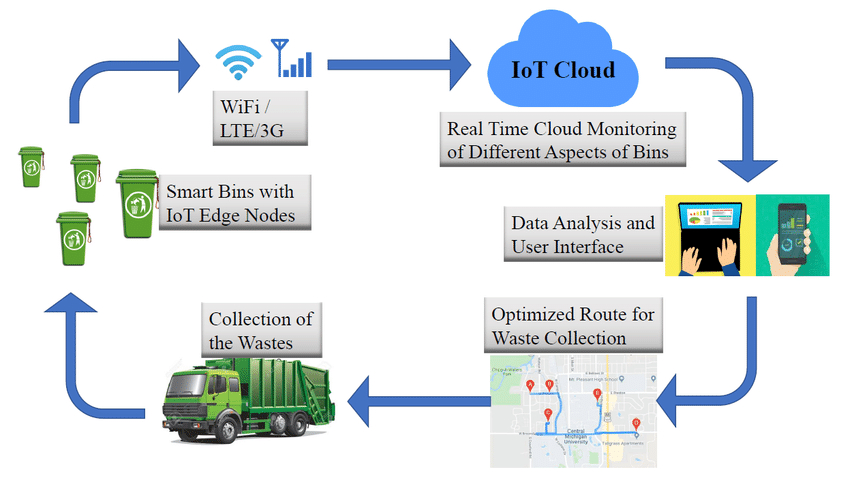
\includegraphics[scale=0.4]{Images/Smart bins.jpg}
\caption{Architektura systému \cite{inproceedings}}
\label{fig:1}
\end{center}
\end{figure}


\section{Automatické třídění}
\label{sec:2}
Automatické třídění se dělí na dvě kategorie, a to přímé a nepřímé. Přímé metody využívají vlastností tříděného materiálu jako je například magnetičnost, elektrická vodivost a podobně. Druhou kategorii jsou metody nepřímé. Ty se spoléhají na senzory, díky kterým dokážou rozpoznat materiál a polohu, která dále slouží robotům či automatickým strojům pro jejich další manipulaci. Těmto metodám se bude více zaobírat v dalších kapitolách \cite{GUNDUPALLI201756}.
\begin{figure}[H]
\begin{center}
\includegraphics[scale=0.6]{Images/přehled.jpg}
\caption{Přehled metod třídění \cite{GUNDUPALLI201756}}
\label{fig:1}
\end{center}
\end{figure}

\subsection{Druhy přímého třídění}
\label{subsec:1}
\subsubsection*{Třídění měkkých (organických) materiálů}
Jak již bylo zmíněno v předchozí kapitole, tyto metody využívají vlastností tříděného materiálu. První z těchto vlastností je tuhost. Na tomto principu jsou založeny metody jako například třídění diskovým sítem či tříděním šroubovým lisem, které jsou určeny pro separaci měkkého (často organického) materiálu od tvrdého \cite{GUNDUPALLI201756} \cite{jank2015waste} \cite{hansen2007effects}. \\

\begin{figure}[H]
\begin{center}
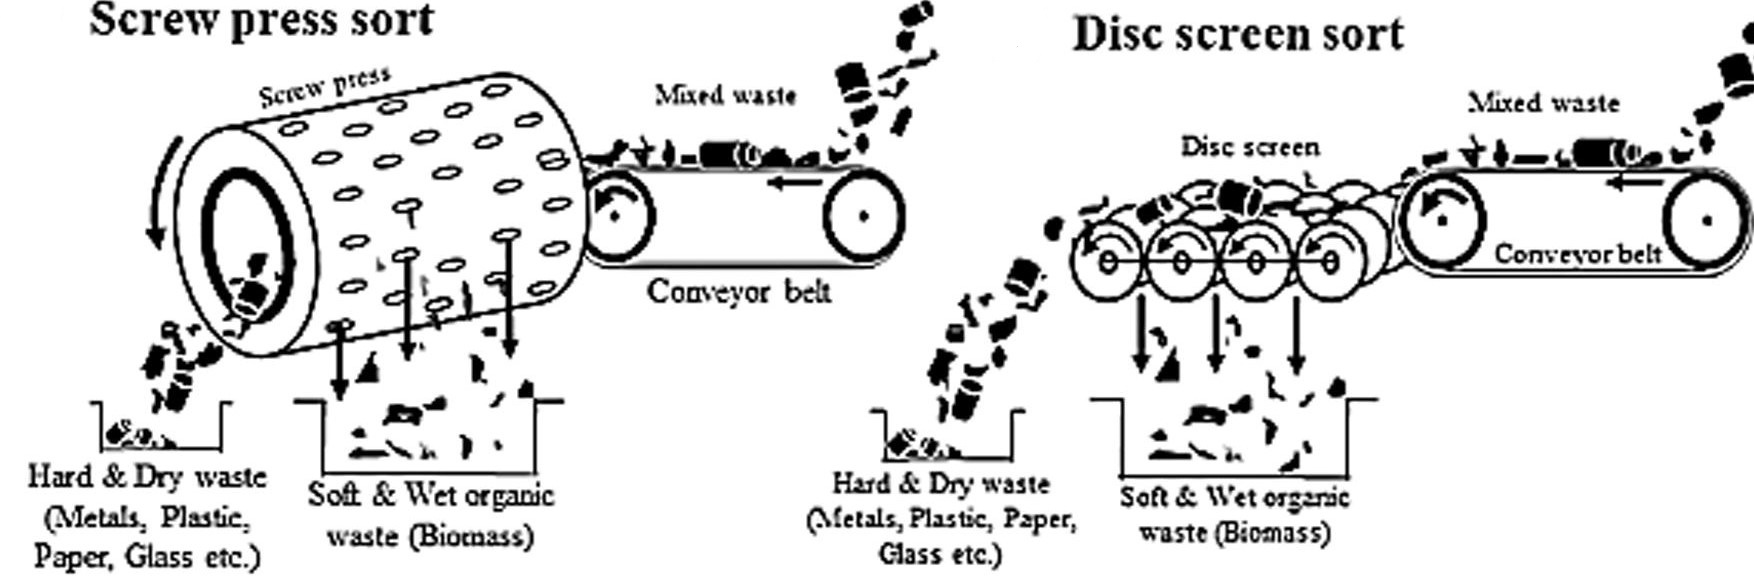
\includegraphics[scale=0.2]{Images/Organic.jpg}
\caption{Třídění měkkých (organických) materiálů \cite{inproceedings}}
\label{fig:1}
\end{center}
\end{figure}

\subsubsection*{Třídění magnetických materiálů}
Další skupinka se zaměřuje na třídění metalického odpadu, jako je například tříděním magnetickým bubnem či pomocí vířivých proudů. V tomto případě je často vhodné použití i drtiče, který tříděný materiál zpracuje na menší části, čímž zlepší výslednou kvalitu třídění \cite{GUNDUPALLI201756} \cite{hansen2007effects} \cite{bonifazi2012recycling}.\\

\begin{figure}[H]
\begin{center}
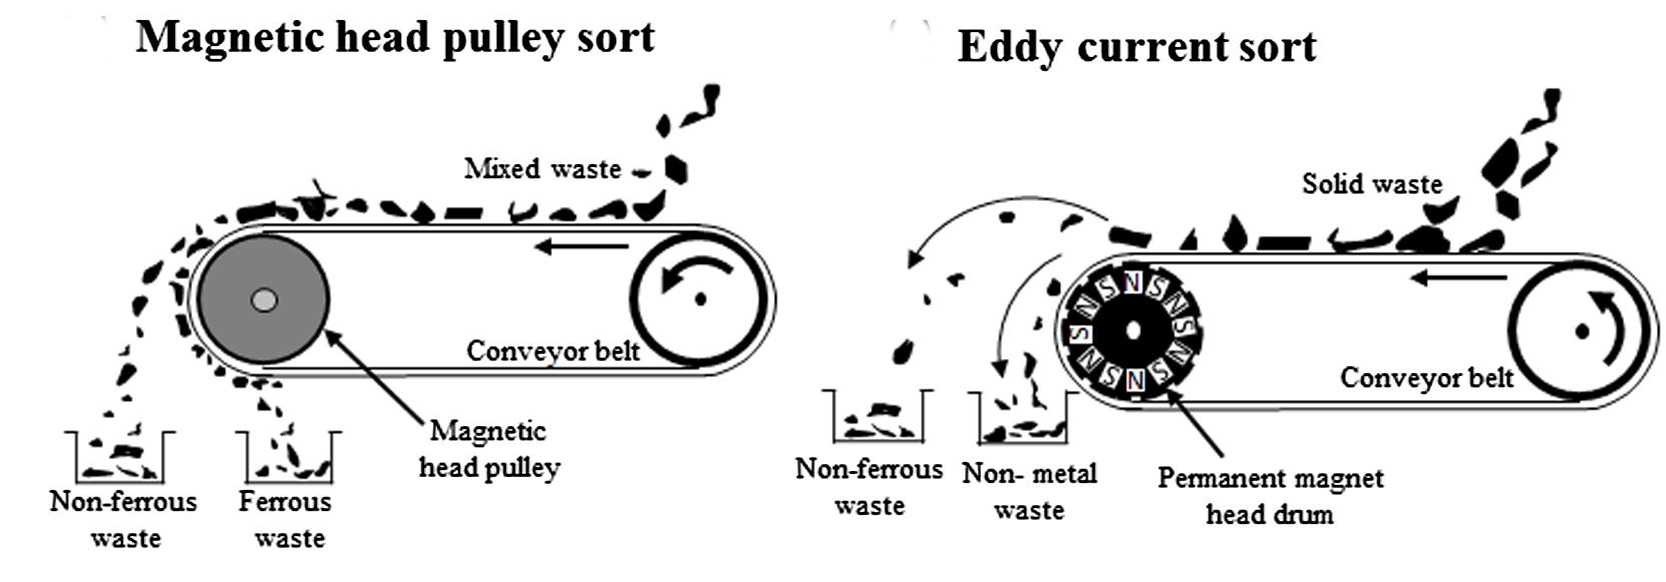
\includegraphics[scale=0.95]{Images/Magnet.jpg}
\caption{Třídění magnetických materiálů \cite{inproceedings}}
\label{fig:1}
\end{center}
\end{figure}

\newpage
\subsubsection*{Třídění plastových materiálů}
Nejpočetnější skupinou jsou metody na třídění plastů. Prvním zástupcem je triboelektrostatická separace, která funguje na principu kontaktní elektrifikace (tribolestickém jevu). Když třízený materiál putuje tribokomorou, drcený plast přítomný v odpadu se nabíjí s různou polaritou třecí elektrifikací. Nabité kusy tohoto odpadu pak procházejí elektrickým polem k jejich oddělení. Trajektorie každého kusu odpadu je určena množstvím neseného náboje. Toto pole pak bývá navrženo tak, aby po průchodu částečky plastu padali do příslušných kontejnerů \cite{GUNDUPALLI201756} \cite{li2015tribo}.\\

\begin{figure}[H]
\begin{center}
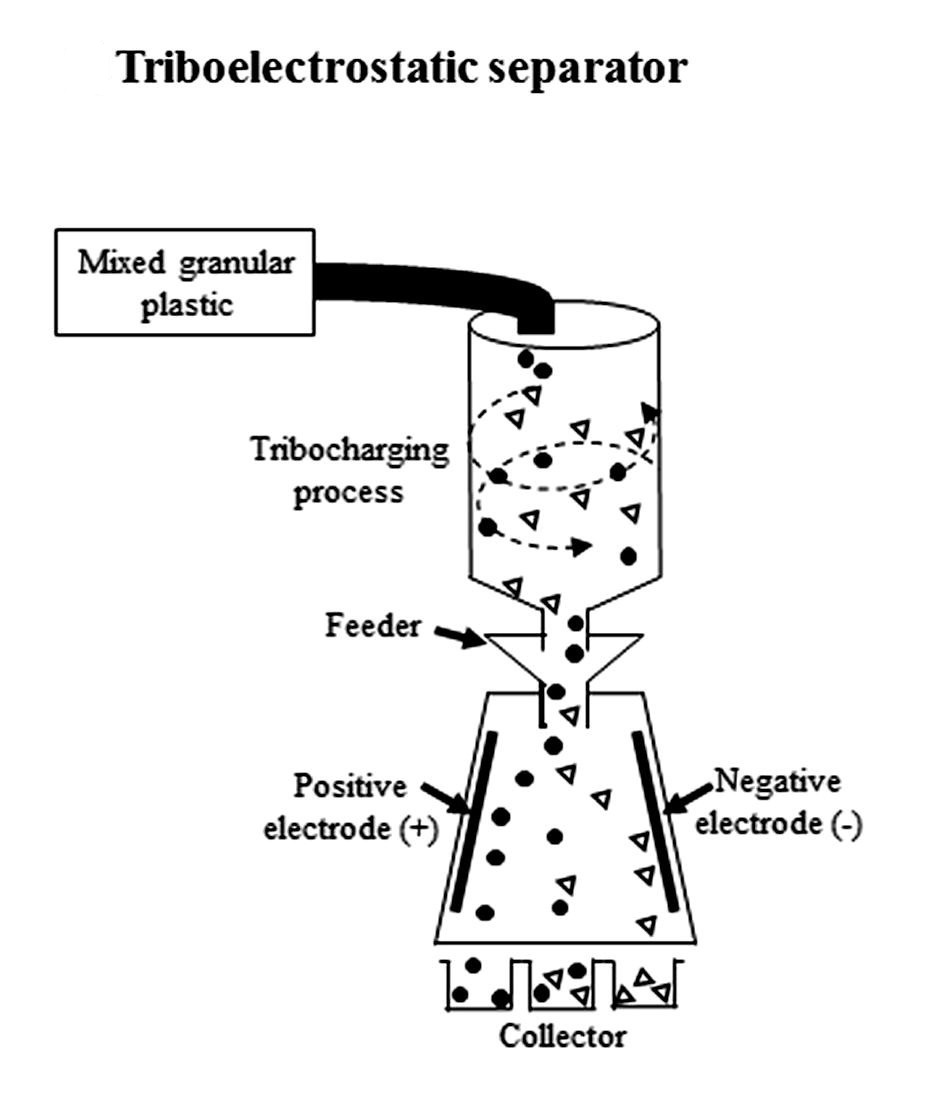
\includegraphics[scale=0.23]{Images/Tribo.jpg}
\caption{Triboelektrostatická separace \cite{inproceedings}}
\label{fig:1}
\end{center}
\end{figure}

Další metodou je hydrocyklon, který pro třídění využívá odstředivou sílu pro hustotní separaci, toto třídění pak ovlivňuje spoustu faktorů jako například kolísání hustoty (od plniv, pigmentů, pórovitosti atd.), smáčivost, tvarové faktory částic se zmenšenou velikostí a míra uvolňování z jiných materiálů \cite{GUNDUPALLI201756} \cite{richard2011optimization} .\\

\begin{figure}[H]
\begin{center}
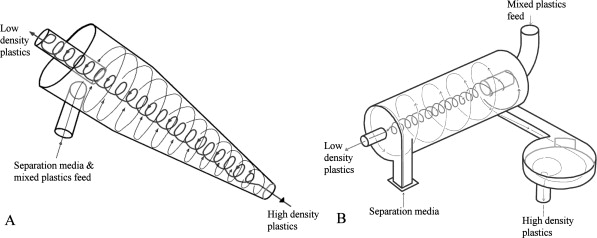
\includegraphics[scale=0.91]{Images/Hydrocyklon.jpg}
\caption{Třídění hydrocyklonem \cite{richard2011optimization}}
\label{fig:1}
\end{center}
\end{figure}

\newpage
Poslední metoda je pomocí flotace, která využívá hydrofobnosti plastu k jeho oddělení z odpadní vody. Při tomto procesu se vzduch rozpouští ve směsi vody a odpadní drti pod vysokým tlakem. Rozpuštěný vzduch se pak uvolňuje do flotační sekce za atmosférického tlaku. To vede k tvorbě pěny na povrchu směsi voda-odpad. Suspendované plastové částice se díky své hydrofobnosti přichytí k těmto bublinám v pěně. Kombinovaná měrná hmotnost bublin nesoucích plastové částice je menší ve srovnání s kapalným médiem, což vede k flotaci \cite{GUNDUPALLI201756} \cite{wang2015flotation}.\\

\begin{figure}[H]
\begin{center}
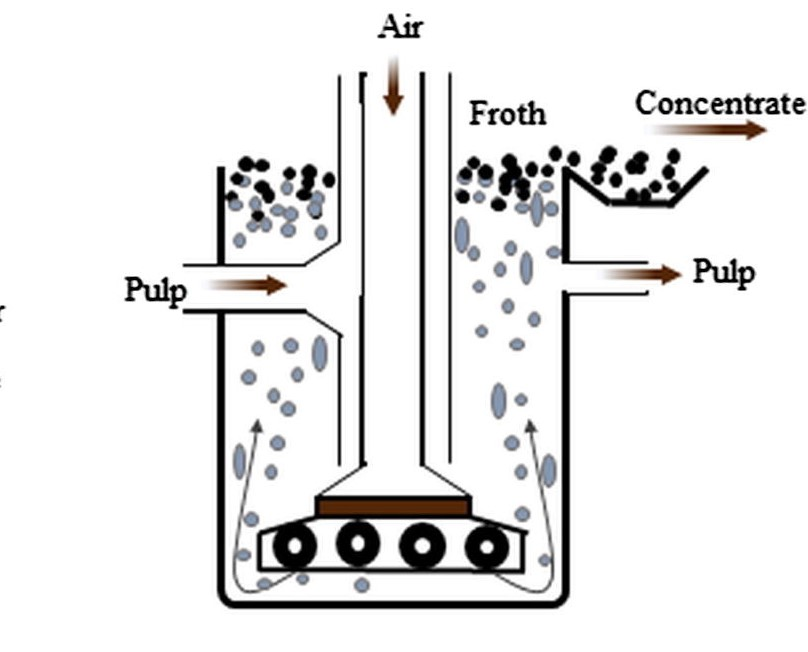
\includegraphics[scale=1]{Images/Flotace.jpg}
\caption{Třídění flotací \cite{inproceedings}}
\label{fig:1}
\end{center}
\end{figure}



\subsection{Druhy nepřímého třídění}
\label{subsec:1}
\subsubsection*{Třídění založené na vířivých proudech}
Funguje na principu magnetického toku, generovaným elektromagnetickou cívkou, který prochází tříděným materiálem, ve kterém se indikuje vířivý proud. Právě přivedením proudu do cívky nad dopravníkem vzniká v axiálním směru cívky primární magnetický tok. Ten pak způsobuje generování vířivých proudů, které působí podle Lenzova zákona proti sekundárnímu magnetickému toku. Proto měřením sekundárního magnetického toku jsme schopni detekovat železný odpad. Ten je pak dále vystřižen například pomocí stlačeného vzduchu
\cite{GUNDUPALLI201756}.

\begin{figure}[H]
\begin{center}
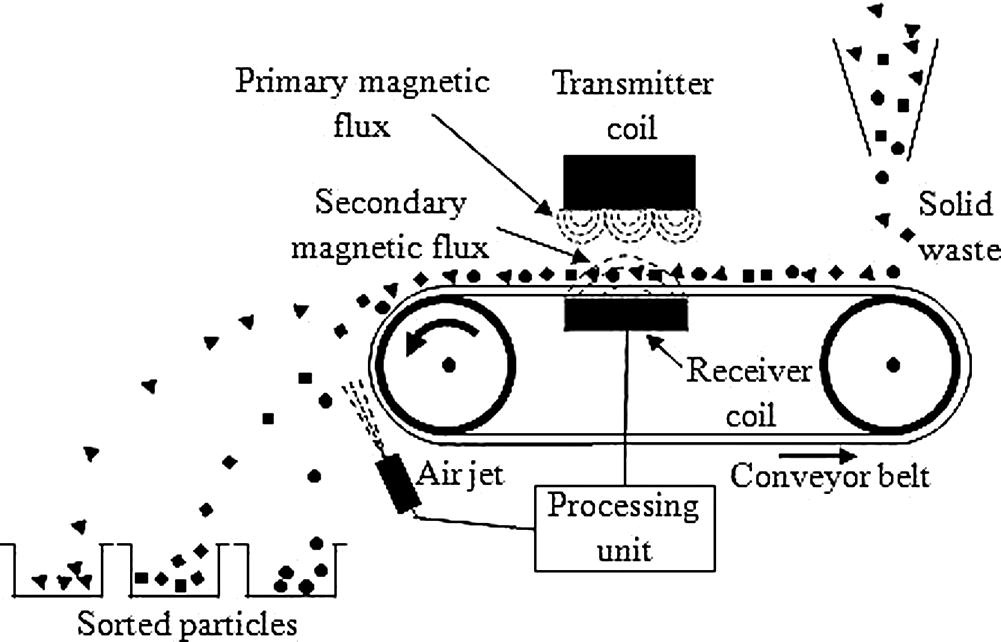
\includegraphics[scale=1.1]{Images/Vířivé proudy.jpg}
\caption{Třídění založené na vířivých proudech \cite{GUNDUPALLI201756}}
\label{fig:1}
\end{center}
\end{figure}

\newpage
\subsubsection*{Spektrometrie laserem buzeného plazmatu (LIBS)}
Systém je založen na použití velmi výkonného laserového pulsu. Ten je přiveden na tříděný materiál, to zapříčiní ablaci tohoto materiálu, který vede k vytvoření plasmových válečků. Následně je záření emitované z této ablatované části zachycováno CCD spektrometrem. Tato metoda má oproti metodě vířivých proudů vyšší rychlost analyzování. Nevýhodou pak však je, že odpad musí být bez maziv, barev a oxidačních vrstev \cite{GUNDUPALLI201756} \cite{solo2004evaluation}.

\begin{figure}[H]
\begin{center}
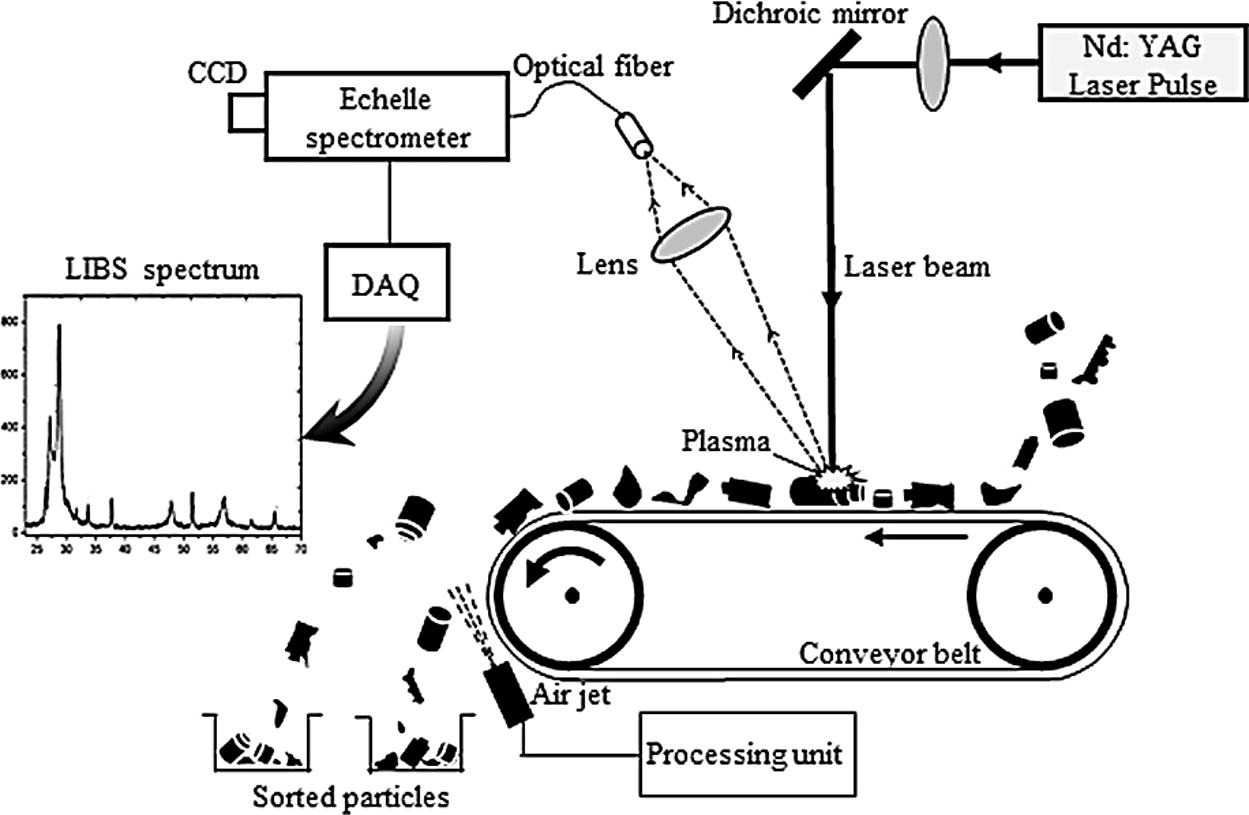
\includegraphics[scale=0.85]{Images/LIBS.jpg}
\caption{Spektrometrie laserem buzeného plazmatu (LIBS) \cite{GUNDUPALLI201756}}
\label{fig:1}
\end{center}
\end{figure}

\subsubsection*{Třídění za pomocí rentgenu}
Funguje na principu pořizování rentgenových snímku a to v řádu několika milisekund. Snímání se dá pak rozdělit na dva typy. Metoda Dual Energy X-ray Transmission (DE-XRT), které spočívá v prosvicování materiálu. Druhá metoda X-ray Fluorescence (XRF) spočívá pak ozáření materiálu a následného snímání odrazu \cite{GUNDUPALLI201756}.

\begin{figure}[H]
\begin{center}
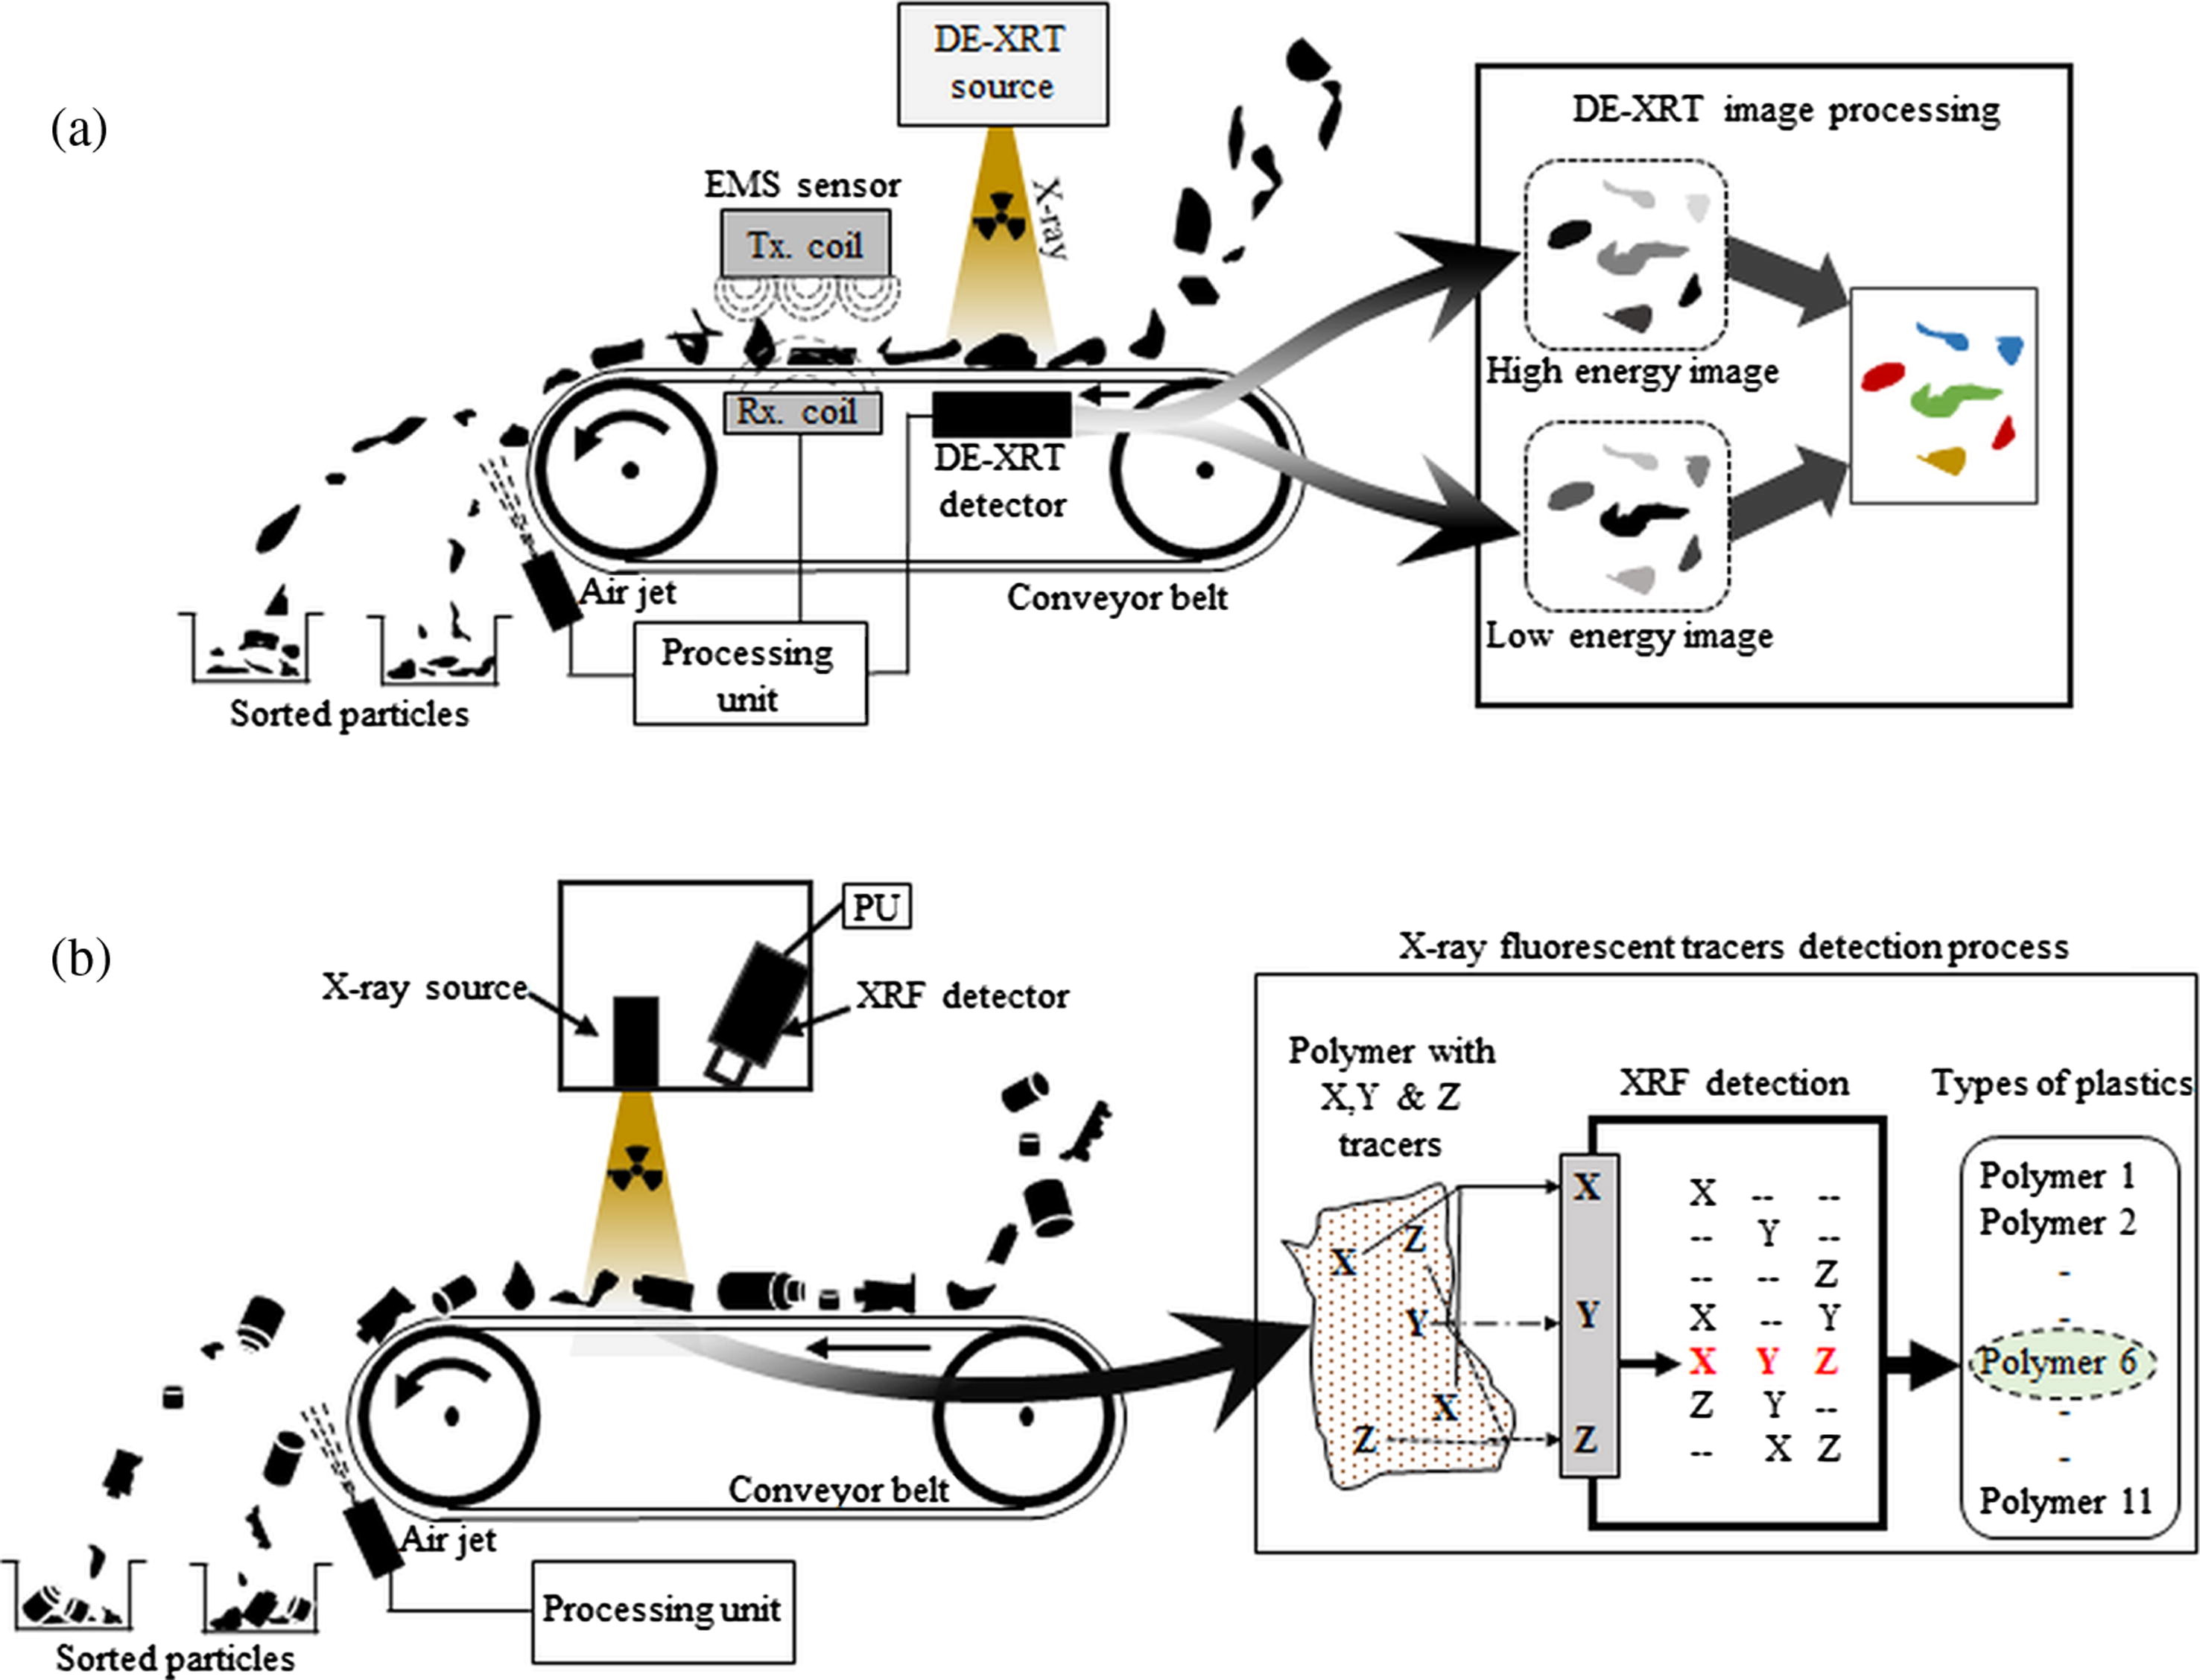
\includegraphics[scale=0.75]{Images/X-ray.jpg}
\caption{Třídění za pomocí rentgenu \cite{GUNDUPALLI201756}}
\label{fig:1}
\end{center}
\end{figure}

\newpage
\subsubsection*{Třídění na optické bázi}
Tato metoda se na rozdíl od předešlých nezaměřuje na fyzické vlastnosti materiálu, ale na vizuální/hmatové podměty jako je například barva, textura či tvar. Jako senzory zde slouží kamery \cite{GUNDUPALLI201756}.

\begin{figure}[H]
\begin{center}
\includegraphics[scale=0.8]{Images/optické.jpg}
\caption{Třídění na optické bázi \cite{GUNDUPALLI201756}}
\label{fig:1}
\end{center}
\end{figure}

\subsubsection*{Třídění založené na spektrálním zobrazování}
Tato metoda kombinuje spektrální zobrazení pomocí CCD kamer s následným zpracováním takto vniklých obrázků různým algoritmy pro rozpoznání materiálu \cite{GUNDUPALLI201756}.

\begin{figure}[H]
\begin{center}
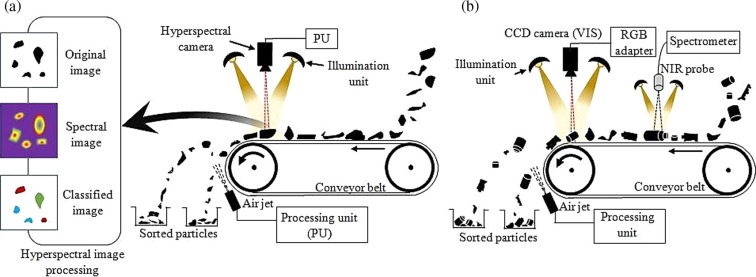
\includegraphics[scale=0.8]{Images/spektrální.jpg}
\caption{Třídění založené na spektrálním zobrazování \cite{GUNDUPALLI201756}}
\label{fig:1}
\end{center}
\end{figure}


%%\section{Ukázka robotizovaného třídění}
%%\label{sec:2}


\section{Závěr}
\label{sec:2}
Tato práce se zabývala v první části automatizovaným sběrem odpadu pomocí IoT chytré popelnice, které celý proces zefektivňuji díky odesíláním dat o míře zaplnění, které se dále využívají pro plánování cest vozů pro sběr odpadu, což má za následek, optimálnější trasu těchto vozidel, tedy i snížení spotřeby, ceny a nižší uhlíkovou stopu. Druhá část se pak zabývá metodami třídění odpadu, ať už metodami přímými, založených na vlastnostech materiálu, či metodami nepřímí, které se spoléhají na senzory. 

% Zdroje
%
\newpage
\begingroup
\makeatletter
\renewcommand\section{\@startsection {section}{1}{\z@}%
                                   {-3.5ex \@plus -1ex \@minus -.2ex}%
                                   {4.5ex \@plus.2ex}%
                                   {\large\bfseries}}
\makeatother

\renewcommand\refname{Zdroje}
\bibliography{reference}
\bibliographystyle{acm}
\endgroup

\end{document}